\documentclass[a4paper]{article}
\usepackage[utf8]{inputenc}
\usepackage{alphabeta}
\usepackage{graphicx}
\usepackage[section]{placeins}
\usepackage{float}
\usepackage{amsmath}
\usepackage{listings}
\usepackage{xcolor}
\usepackage{amsmath}
\usepackage{extarrows}
\usepackage{amssymb}
\usepackage{verbatim}
\usepackage{enumerate}
\usepackage{eurosym}

\definecolor{codegreen}{rgb}{0,0.6,0}
\definecolor{codegray}{rgb}{0.5,0.5,0.5}
\definecolor{codepurple}{rgb}{0.58,0,0.82}
\definecolor{backcolour}{rgb}{0.95,0.95,0.92}

\lstdefinestyle{mystyle}{
    backgroundcolor=\color{backcolour},   
    commentstyle=\color{codegreen},
    keywordstyle=\color{magenta},
    numberstyle=\tiny\color{codegray},
    stringstyle=\color{codepurple},
    basicstyle=\ttfamily\footnotesize,
    breakatwhitespace=false,         
    breaklines=true,                 
    captionpos=b,                    
    keepspaces=true,                 
    numbers=left,                    
    numbersep=5pt,                  
    showspaces=false,                
    showstringspaces=false,
    showtabs=false,                  
    tabsize=2
}

\lstset{style=mystyle}

\setlength{\parindent}{0pt}
\setlength{\parskip}{1em}
\setlength{\jot}{4mm}

\title{Συστήματα Μικροϋπολογιστών \\ 1η ομάδα ασκήσεων}
\author{Νικόλαος Παγώνας, el18175 \and Αναστάσιος Παπαζαφειρόπουλος, el18079}
\date{}

\begin{document}

\maketitle

\section*{1η άσκηση}

Για την μετατροπή σε assembly χρησιμοποιήθηκε ο πίνακας 2 του παραρτήματος 2 των σημειώσεων. Πρέπει να προσέξουμε ότι στις διευθύνσεις δίνεται πρώτα το LSByte και ύστερα το MSByte. Για παράδειγμα, όταν σε γλώσσα μηχανής διαβάζουμε \textbf{00 30}, αυτό αναφέρεται στην διεύθυνση \textbf{3000Η}. 


\verbatiminput{../files/ex1.txt}

Παρατηρώντας προσεκτικά τον κώδικα, αλλά και επιβεβαιώνοντας με τη χρήση του mLAB, συμπεραίνουμε ότι το πρόγραμμα 

\begin{itemize}

	\item παίρνει είσοδο από τα dip switches (2000Η)
	\item βρίσκει τη θέση του πρώτου bit από τα αριστερά που είναι ίσο με 1 
	\item εμφανίζει τη θέση αυτή σε δυαδική μορφή, στα LED εξόδου (3000Η) 
\end{itemize}

Για να εκτελείται συνεχώς, χρειάζεται μία εντολή jump η οποία επιστρέφει στην αρχή του προγράμματος.

\begin{samepage}
Το διάγραμμα ροής που αντιστοιχεί στο παραπάνω πρόγραμμα:

\begin{figure}[H]
	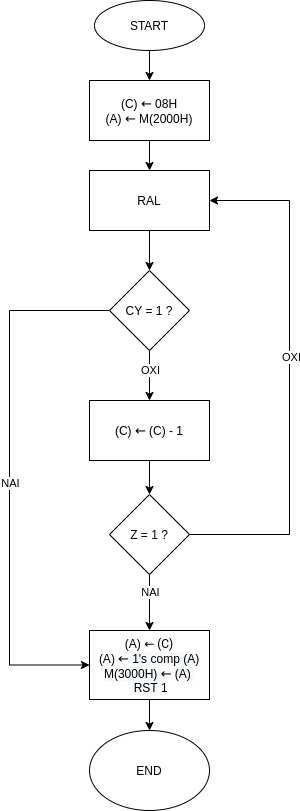
\includegraphics[height=0.85\textheight]{../files/ex1.jpg}
\end{figure}
\end{samepage}
\section*{2η και 3η άσκηση}

Ο κώδικας και των δύο ασκήσεων βρίσκεται στα αρχεία  \texttt{ex2.8085} και \texttt{ex3.8085} αντίστοιχα, μαζί με τα κατάλληλα σχόλια για την κατανόηση της λειτουργίας των προγραμμάτων.

\section*{4η άσκηση}

Αν συμβολίσουμε με x τον αριθμό των τεμαχίων:


\begin{center}
	\def\arraystretch{2.75}
	\begin{tabular}{|c|c|c|}
		\hline
		\text{Τεχνολογία} & Συνολικό Κόστος (\euro) & Κόστος/τεμάχιο (\euro) \\
		\hline 
		1η & $ 20000+20x $ & $ \dfrac{20000}{x}+20 $\\
		\hline 
		2η & $ 10000+40x $ & $ \dfrac{10000}{x}+40 $\\
		\hline
		3η & $ 100000+4x $ & $ \dfrac{100000}{x}+4 $\\
		\hline
		4η & $ 200000+2x $ & $ \dfrac{200000}{x}+2 $\\
		\hline
	\end{tabular}
\end{center}

\begin{samepage}
	Απεικονίζουμε τις καμπύλες κόστους ανά τεμάχιο:
	\begin{figure}[H]
		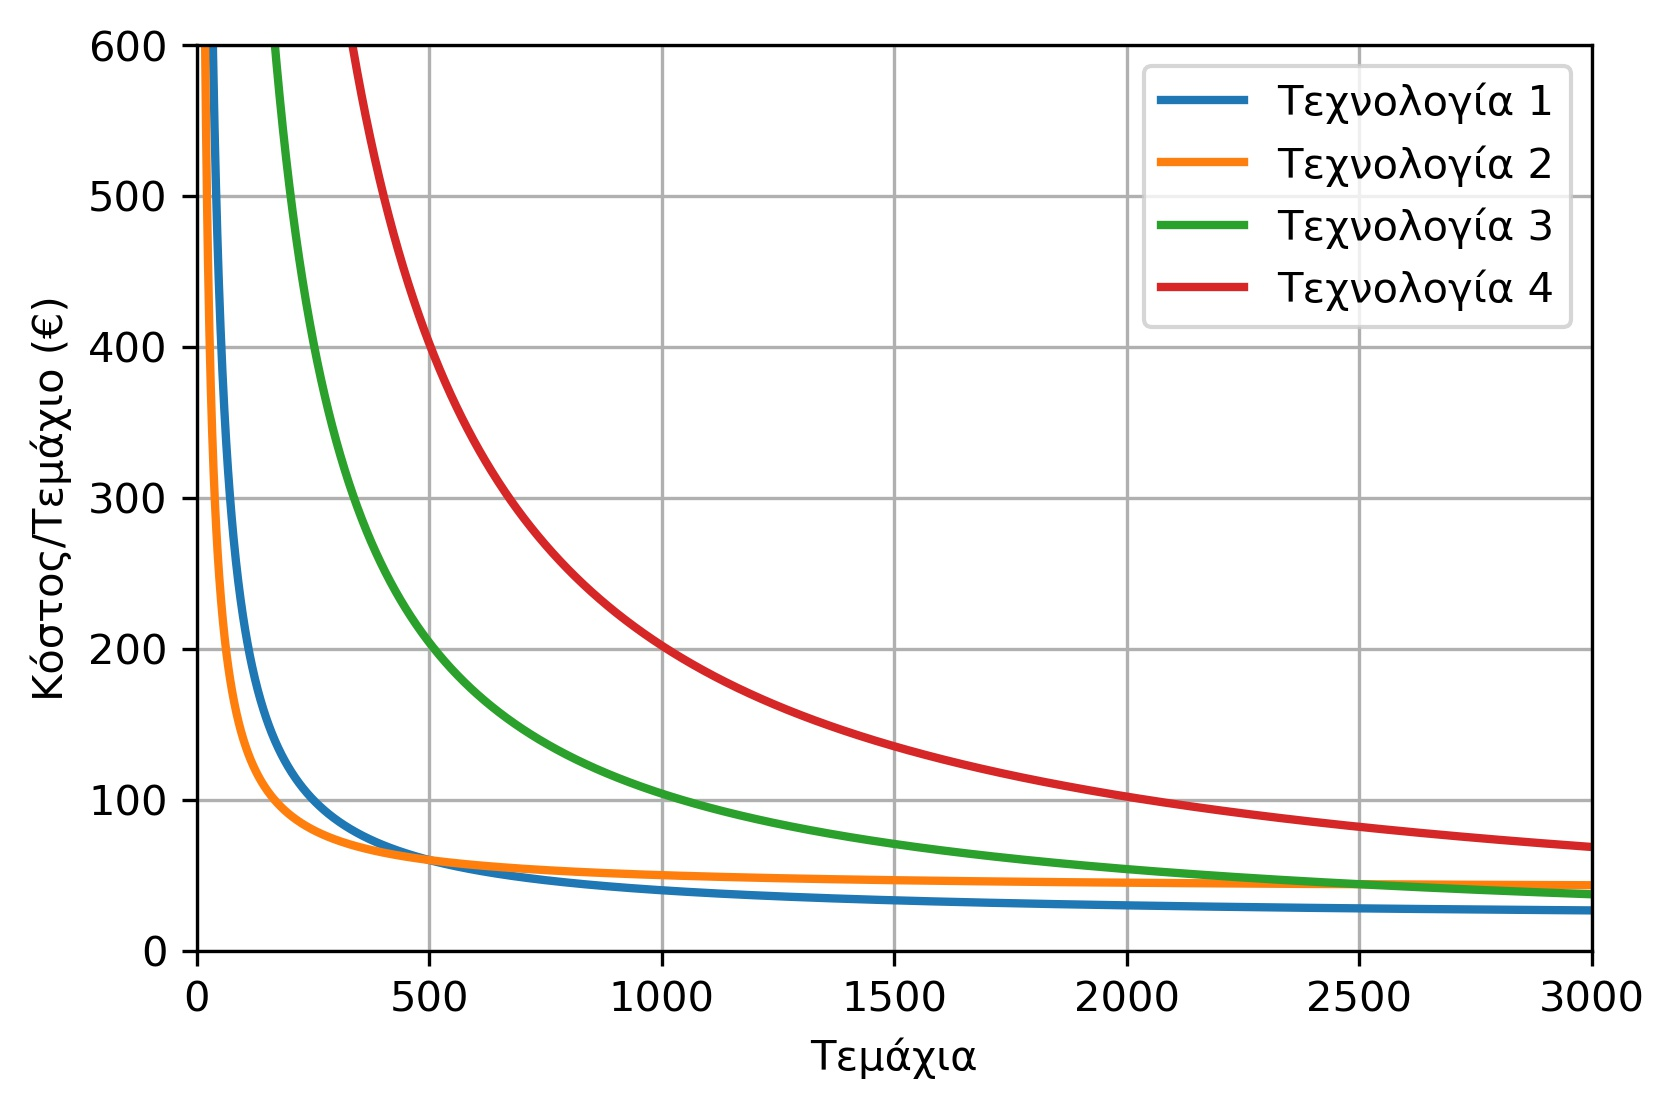
\includegraphics[width=\textwidth]{../files/ex4perunitpython.jpg}
	\end{figure}
	
	Και τις καμπύλες συνολικού κόστους:
	
	\begin{figure}[H]
		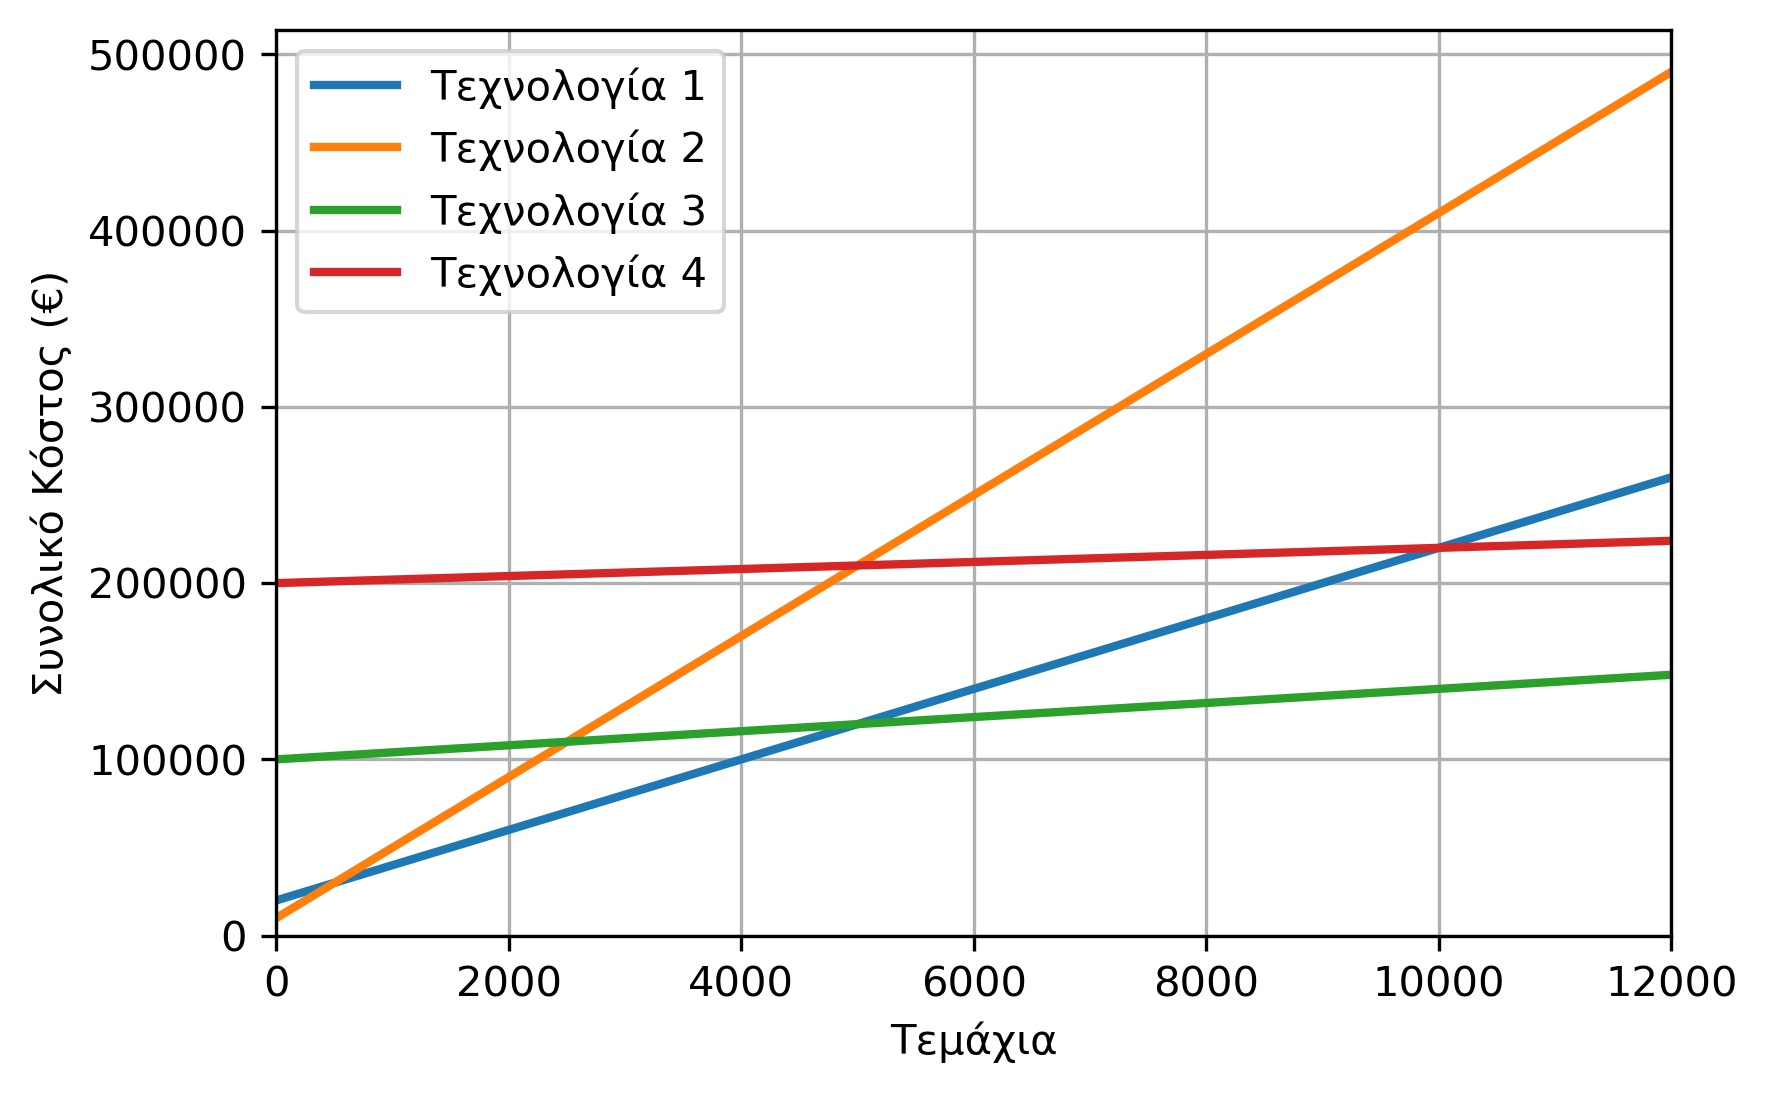
\includegraphics[width=\textwidth]{../files/ex4totalpython.jpg}
	\end{figure}
\end{samepage}
\begin{samepage}
	Επίσης, χρησιμοποιώντας τις εξισώσεις των ευθειών που δίνουν το συνολικό κόστος για κάθε περίπτωση, βρίσκουμε τα σημεία τομής τους, και άρα ποιο κόστος είναι ελάχιστο στο εκάστοτε διάστημα. Προκύπτουν τα εξής:
	
	\begin{itemize}
		\item $ 0 < x < 500 $: Ευνοϊκότερη η 2η τεχνολογία. 
		\item $ 500 < x < 5000 $: Ευνοϊκότερη η 1η τεχνολογία.
		\item $ 5000 < x < 100000 $: Ευνοϊκότερη η 3η τεχνολογία.
		\item $ x > 100000 $: Ευνοϊκότερη η 4η τεχνολογία.
	\end{itemize}
\end{samepage}

Για να εξαφανιστεί η επιλογή της πρώτης τεχνολογίας, πρέπει η 2η τεχνολογία να είναι ευνοϊκότερη ακόμα και στην περιοχή 500 με 5000. Συμβολίζοντας το υπό διερεύνηση κόστος των I.C. της 2ης τεχνολογίας με k:
\begin{align*}
	20000+20x &> 10000 + (k+10)x \\
	k &< \frac{10000}{x}+10 
\end{align*}

Επειδή το παραπάνω πρέπει να ισχύει για $ x \in [500,5000] $, έχουμε:

\begin{itemize}
	\item Για $x = 500, k < 30$
	\item Για $x = 5000, k < 12$
\end{itemize}

Επομένως συνολικά, πρέπει το κόστος I.C. ανά τεμάχιο να είναι μικρότερο από 12 ευρώ προκειμένου να εξαφανιστεί η 1η τεχνολογία.

\section*{5η άσκηση}

\lstinputlisting[language=Verilog]{../files/ex5.txt}



\section*{6η άσκηση}
i)
	\begin{figure}[H]
		\centering
		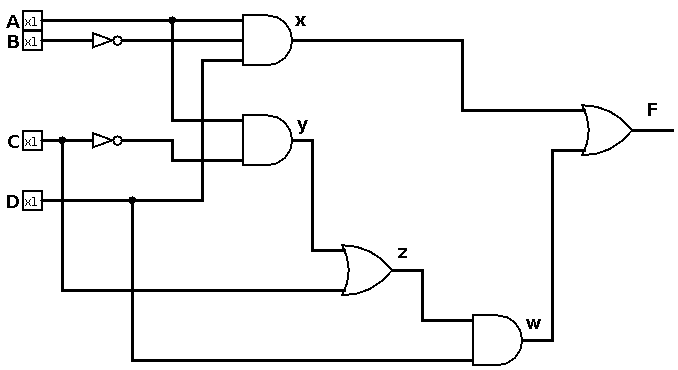
\includegraphics[width=\textwidth]{../files/ex6ia.png}
		\caption{Circuit A}
	\end{figure}
	\begin{figure}[H]
		\centering
		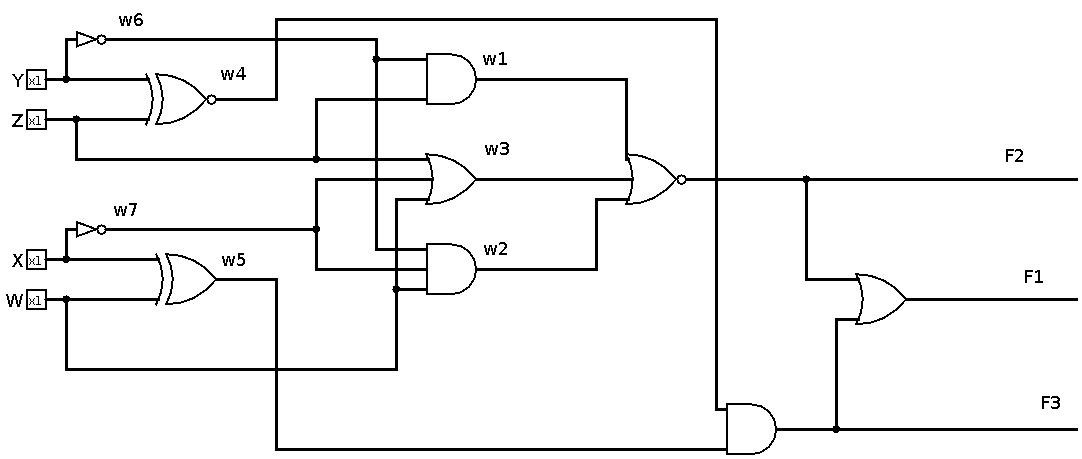
\includegraphics[width=1.1\textwidth]{../files/ex6ib.png}
		\caption{Circuit B}
	\end{figure}
	\begin{figure}[H]
		\centering
		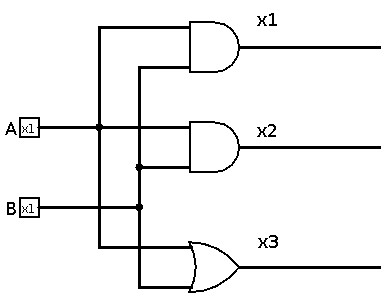
\includegraphics[width=0.5\textwidth]{../files/ex6ic.png}
		\caption{Circuit C}
	\end{figure}
ii)
\lstinputlisting[language=Verilog]{../files/ex6ii.txt}
iii)
\lstinputlisting[language=Verilog]{../files/ex6iii.txt}

\section*{7η άσκηση}

Κωδικοποιούμε τις καταστάσεις των αυτομάτων ως εξής:
\begin{align*}
	a \rightarrow 00 \\
	b \rightarrow 01 \\
	c \rightarrow 10 \\
	d \rightarrow 11 \\
\end{align*}

H είσοδος συμβολίζεται με x και η έξοδος με y.
Το MSB και το LSB της κατάστασης με A και B αντίστοιχα.
Έτσι, έξοδος y για το αυτόματο Mealy είναι η εξής:

\begin{center}
	\begin{tabular}{|c|c|c||c|}
		\hline
		A & B & x & y \\
		\hline
		0 & 0 & 0 & 1 \\
		\hline
		0 & 0 & 1 & 0 \\
		\hline
		0 & 1 & 0 & 1 \\
		\hline
		0 & 1 & 1 & 0 \\
		\hline
		1 & 0 & 0 & 1 \\
		\hline
		1 & 0 & 1 & 0 \\
		\hline
		1 & 1 & 0 & 0 \\
		\hline
		1 & 1 & 1 & 1 \\
		\hline
	\end{tabular}
\end{center}

H απλοποίηση με χάρτη Karnaugh δίνει: $ y = ABx+A'x'+B'x' $

Αντίστοιχα, για την έξοδο του αυτομάτου Moore ισχύει:

\begin{center}
	\begin{tabular}{|c|c||c|}
	\hline
	A & B & y \\
	\hline
	0 & 0 & 0 \\
	\hline
	0 & 1 & 1 \\
	\hline
	1 & 0 & 1 \\
	\hline
	1 & 1 & 0 \\
	\hline
	\end{tabular}
\end{center}

Έχουμε $ y = AB'+A'B = A \ \text{XOR} \ B $ 

Έτσι, η υλοποίηση σε Verilog για τα δύο αυτόματα είναι η εξής:

\lstinputlisting[language=Verilog]{../files/ex7.txt}
\end{document}
